\hypertarget{ux5927ux6a21ux578bux667aux80fdux4f53}{%
\chapter{大模型智能体}\label{ux5927ux6a21ux578bux667aux80fdux4f53}}

\hypertarget{ux667aux80fdux4f53ux53caux5176ux67b6ux6784}{%
\section{智能体及其架构}\label{ux667aux80fdux4f53ux53caux5176ux67b6ux6784}}

\hypertarget{ux4e00ux667aux80fdux4f53ux6982ux8ff0}{%
\subsection{一、智能体概述}\label{ux4e00ux667aux80fdux4f53ux6982ux8ff0}}

大模型智能体（LLM Agent），是以LLM为核心，搭建起的一个能与用户和外部环境互动（LLM本身不能自主与外部环境互动），自主感知、执行任务并获取反馈的智能体。它让LLM的能力不仅限于传统意义上的``对话''，而是能真正帮助人类在实际环境中完成一定的工作任务。Agent工作流以完整的程序形式呈现，程序中会有输入Prompt、调用LLM、调用工具等不同语句块，以实现整体的Agent功能，需要综合模型推理、工具调用、记忆检索等多方面。完成一次任务时，Agent输出文本思考或动作，当输出动作与环境交互后，环境反馈又会被输入Agent继续思考处理。

一个完整的Agent（智能体）应包含以下模块：

推理模块：大语言模型，可以生成动作指令。

记忆或知识库模块：除了上下文窗口（下面会解释）外，目前记忆或知识库一般外置于模型。模型可通过检索增强生成（RAG）方法，调用记忆或知识库中的内容进行生成。

工具调用模块：模型与环境互动的核心接口，模型通过工具调用，在环境中执行行动、获得反馈。

上下文Agent即每次的输入。和LLM的上下文仅包括提示词和前面已经生成的内容不同，Agent的上下文还包括（可能经过压缩后的）环境反馈，如工具调用结果、检索结果，还可能有从记忆中提取的内容。因此，Agent时代的范式正在从Prompt Engineering走向Context Engineering。Agentic RL中，马尔可夫性环境中Agent所处的``状态''也包括以上所有上下文的组成部分，即对于完成同一个任务中的第t+1次输入（第t+1轮对话）：

上下文注入与状态转移（Context Injection / State Transition）：将动作 \(a_t\) 和反馈 \(o_{t+1}\) 拼接（记为 \(\oplus\)）到现有上下文中，完成所谓的``瞬间转移''，形成新的决策状态：

\[
h_{t+1}=h_t \oplus a_t \oplus o_{t+1}
\]

\hypertarget{ux4e8creactux8303ux5f0f}{%
\subsection{二、ReAct范式}\label{ux4e8creactux8303ux5f0f}}

结合外部程序和提示词，让模型交替进行思考、行动、观察（相当于人类的思考、行动、感知）。其中行动指从外部搜索信息、输出最终回答等，可能涉及调用外部工具（大模型会生成调用该工具所需的精确指令或参数）；观察指处理本步行动后得到的信息或观察环境的变化。思考过程中，如输出特定token，则调用工具开始行动或中止循环（后来的一些改进架构中，把直接中止循环变为交给特定检查机制检查任务是否完成）。

举一个例子：

问题 科罗拉多造山带东部区域延伸到的区域的海拔范围是多少？

思考 1 我需要搜索科罗拉多造山带，找到科罗拉多造山带东段延伸的区域，然后找到该区域的海拔范

围。

操作 1 搜索 {[}科罗拉多造山带{]}

观察 1 科罗拉多造山带是科罗拉多及其周边地区造山运动的一段。

思考 2 它没有提到东部地区。所以我需要查一下东部地区。

操作 2 查找 {[}东部地区{]}

观察 2 (结果 1 / 1) 东部区域延伸至高平原，称为中原造山带。

思考 3 科罗拉多造山运动的东部区域延伸到高平原。所以我需要搜索高平原，找到它的海拔范围。

操作 3 搜索 {[}高平原{]}

观察 3 高平原指的是两个截然不同的陆地区域之一。

思考 4 我需要搜索高平原（美国）

操作 4 搜索 {[}高平原（美国）{]}

观察 4 高平原是大平原的一个分区。从东到西，高平原的海拔从 1800 到 7000 英尺 (550 到

2130 米) 不等。

思考 5 高平原海拔高度从 1800 到 7000 英尺，所以答案是 1800 到 7000 英尺。

操作 5 结束 {[}1800 到 7000 英尺{]}

当然，以上是要求模型必须在输出前面加上``思考/操作/观察''的原始ReAct，后来也出现了基于ReAct的变体，并非都有这样的硬性要求，但这三个阶段构成循环的核心思想不变。如OpenAI Codex：

假设在终端里输入：给项目的README.md加一个架构图。

第一步：构建Prompt

Codex先构建一个Prompt，包括System Prompt（告诉模型它是谁、能干什么）， Tools（有哪些工具可以调用），Context（环境上下文如当前在哪个目录、用的什么shell），对话或输出历史，和用户指令。

第二步：模型推理（Inference）

Codex把这个Prompt发给模型，模型做出决定：调用shell工具，执行catREADME.md。

第三步：工具调用（ToolCall）

Codex收到模型的请求，在本地执行命令，把README.md的内容读出来。

第四步：结果反馈（FeedBack）

终端把README.md的内容吐了出来。对于循环架构而言，这并不意味着结束。Codex把命令的输出追加到Prompt里，再发给模型。

循环（Agent Loop）

模型看到了README的内容，再次进行推理：可能是生成一个Mermaid图，可能是直接写一段ASCII图形\ldots\ldots 然后再调用工具写入文件。这个循环一直持续，直到模型认为任务完成了，输出一条结束信息。Agent会自己检查错误、验证结果等，真正成为可持续工作的智能体。

\hypertarget{ux4e09ux5148ux8ba1ux5212ux540eux6267ux884c}{%
\subsection{三、先计划，后执行}\label{ux4e09ux5148ux8ba1ux5212ux540eux6267ux884c}}

在完成复杂的任务时，先计划后执行往往准确率更高，如Cursor、Claude Code等均有Plan Mode，用Prompt要求其先制定计划，再通过ReAct范式执行。同时，也可以动态维护计划，在每次行动后，也可以根据观察到的反馈和执行情况更新计划。

这种架构依赖于合理的规划，对于复杂的任务规划难度可能较大。因此，在Claude Code等Agent中，制定计划已经不是一次性的任务，而也是一个循环：在``只读模式''下，模型构成``推理规划---阅读或向用户询问''的闭环，在阅读文件及和用户的交互中不断修改规划。

\hypertarget{ux56dbux81eaux7701ux4e0eux53cdux601d}{%
\subsection{四、自省与反思}\label{ux56dbux81eaux7701ux4e0eux53cdux601d}}

在ReAct的基础上增加反思步骤，Agent执行失败或结果不理想时会生成一段自我批评（Self-Reflection），并将这个批评作为短期记忆存储起来，在下一次尝试时提醒自己不要重蹈覆辙。这大幅提升了复杂任务的成功率，无需重新训练模型。

\hypertarget{ux4e94ux81eaux4e3bux5faaux73af}{%
\subsection{五、自主循环}\label{ux4e94ux81eaux4e3bux5faaux73af}}

我们希望构建能自主循环的智能体，能根据总目标，独立设定子目标、制定计划并持续执行。它的工作流是一个可持续自主运行的循环，可以动态衡量与目标的差距、进行反思、生成新子任务、调整执行子任务的顺序等，直至完成目标。挑战在于，可能逐渐偏离原始目标，需要纠偏机制；需要设立合理的终止判断机制；持续运行成本较大；可解释性弱，甚至可能存在安全风险。

\hypertarget{ux516dralgh-loop}{%
\subsection{六、Ralgh Loop}\label{ux516dralgh-loop}}

2025年底，澳大利亚前程序员Geoffrey Huntley编写了5行代码：while :; do cat prompt.md \textbar{} claude-code ; Done并让AI自动运行这个循环，最终取得了惊人的效果。该循环被称为Ralph Loop，是一种AI Agent自动化循环工作流。将AI置于一个while(true)循环中，给AI指定一个任务，以及一个可编程客观验证的``完成标志''（如输出特定字符串、通过特定测试案例、返回0错误码）。AI完成任务后尝试退出，如果没有检测到完成标志，Stop Hook脚本会拦截退出，并把同一个提示词再次送入系统，开启一个全新的会话重新解决，此时AI可以看到自己的上轮输出、错误日志或Git历史，但不保留上一轮的其他上下文，这样也避免了上下文溢出。从而这样可以形成一个自我反馈闭环，每一轮AI不断尝试解决问题，直至全部成功。

Ralph Loop可以让我们解决许多普通AI工具会崩溃的痛点。大多数人使用AI编程工具时，只有一个想法，但任务太大了，AI在上下文窗口内无法一次性解决。而Ralph不强求一次性解决问题，就意味着我们可以让AI先制定计划，然后在一个循环中，把所有事情拆到``AI一次就能做完、一次就能判断对错''的最小颗粒度。具体而言，可以分为以下步骤：

\begin{enumerate}
\def\labelenumi{\arabic{enumi}.}
\item
  输入明确的指令。
\item
  让AI拆解任务，转化为需求清单，每个任务都需要一个明确的检查方式来判断是否成功。如：``增加一个优先级列，默认为中等。''``下拉菜单显示选项：全部、高、中、低''，而不是用``好看''这种模糊的表述。需求的描述直接决定输出结果的好坏。
\item
  运行Ralgh循环。
\end{enumerate}

\hypertarget{ux53c2ux8003ux6587ux732e-115}{%
\subsection{参考文献}\label{ux53c2ux8003ux6587ux732e-115}}

\begin{itemize}
\tightlist
\item
  《动手学大模型智能体》。
\end{itemize}

\clearpage

\hypertarget{ux63d0ux793aux5de5ux7a0b}{%
\section{提示工程}\label{ux63d0ux793aux5de5ux7a0b}}

\hypertarget{ux4e00ux57faux672cux6982ux5ff5}{%
\subsection{一、基本概念}\label{ux4e00ux57faux672cux6982ux5ff5}}

提示词是输入给大语言模型或智能体的一段语言指令，我们通过输入提示来明确希望模型完成的任务及其要求。提示词一般分为两类。

\begin{enumerate}
\def\labelenumi{\arabic{enumi}.}
\item
  系统提示：向大语言模型提供的一组初始指令或背景信息，用于指导智能体的行为方式和响应模式，设定其角色、语气和知识范围等。
\item
  用户提示：是用户输入的问题、请求或命令，旨在获取大语言模型的具体回应或完成特定任务，是触发大语言模型智能体产生回复的直接原因。
\end{enumerate}

在多轮问答时，将不变的规则放入系统提示，变化的规则放入用户提示中会方便许多。

\hypertarget{ux4e8cux63d0ux793aux8bcdux5e94ux8be5ux5305ux62ecux7684ux5185ux5bb9}{%
\subsection{二、提示词应该包括的内容}\label{ux4e8cux63d0ux793aux8bcdux5e94ux8be5ux5305ux62ecux7684ux5185ux5bb9}}

\begin{enumerate}
\def\labelenumi{\arabic{enumi}.}
\item
  任务说明：明确告诉模型你要它完成什么任务。
\item
  背景设定：当前任务、智能体身份或上下文环境。
\item
  输出格式限制：输出格式、风格或字数。
\item
  示例（可选）：给出参考示例，让模型可以模仿。
\end{enumerate}

\hypertarget{ux4e09ux63d0ux793aux8bcdux8bbeux8ba1ux7684ux539fux5219}{%
\subsection{三、提示词设计的原则}\label{ux4e09ux63d0ux793aux8bcdux8bbeux8ba1ux7684ux539fux5219}}

\begin{enumerate}
\def\labelenumi{\arabic{enumi}.}
\item
  清晰：避免模糊不清、存在歧义的指令。
\item
  具体：给出更具体、细节、最好容易判断正确性的限制性要求。
\item
  背景或角色设定：如``假设你是一名经验丰富的医生''，模型就会给出更专业化的医学论断；``假设你是一名资深律师''，模型就会更深入聚焦于法律等。
\item
  适度冗余：特别重要的要求可以反复强调。
\end{enumerate}

\hypertarget{ux56dbux63d0ux793aux5de5ux7a0bux7684ux6280ux5de7}{%
\subsection{四、提示工程的技巧}\label{ux56dbux63d0ux793aux5de5ux7a0bux7684ux6280ux5de7}}

\begin{enumerate}
\def\labelenumi{\arabic{enumi}.}
\tightlist
\item
  思维链（Chain of Thought）
\end{enumerate}

运用Prompt要求模型在生成最终答案之前，先生成一系列模拟人类思考的中间推理步骤，将复杂的推理任务分解为多个更简单、更不易出错的子任务。

为什么有效？

（1）降低认知负荷：~大模型本质上是一个基于概率的序列预测器。直接预测最终答案（如``108''）是一个极其困难的任务，因为从问题到答案的``语义距离''非常远。CoT通过插入中间步骤，将``长距离依赖''转化为多个``短距离依赖''。模型只需要根据上文，预测下一个最合理的推理步骤或符号，这更符合其底层能力。

（2）对齐模型优势：~大模型在海量代码和文本中学到的是语法结构、数学公式、逻辑关系和常识。CoT通过引导模型输出``首先''、``其次''、``根据公式XX''等词语，激活了模型在这些程序性知识和逻辑结构上的强大能力，而不是强迫它去``猜''一个数字。
（3）减少组合泛化错误：~复杂问题是由多个基本概念（如加法、乘法、公式）组合而成。模型可能知道每个基本概念，但组合应用时容易出错。CoT将组合过程显式化，让模型一步步应用这些基本概念，从而提高了正确率。

（4）涌现能力：~CoT是一种典型的涌现能力。在较小的模型（如数亿参数）上，即使使用CoT提示，效果也提升有限。但在大型模型（如超过1000亿参数）上，这种能力会突然变得非常明显和有效。

\begin{enumerate}
\def\labelenumi{\arabic{enumi}.}
\setcounter{enumi}{1}
\item
  上下文学习：通过在输入中添加示例来提高回答质量，更能得到符合要求的回答。上下文学习具体分为零样本（Zero-Shot）、单样本（One-Shot），少样本（Few-Shot）等提示方法。
\item
  自我一致性：多次生成，取出现频率最多的答案作为回答，往往比一次回答更可靠。
\item
  反思提示
\end{enumerate}

我们运用三个模型：

（1）执行者（Actor）：根据状态和观察结果生成文本或动作，在环境中采取动作并观察，得到轨迹。记忆组件用于提供额外的上下文信息，例如曾经的错误。

（2）评估者（Evaluator）：对执行者的输出进行评估，对执行者根据其动作轨迹给予一定奖励。

（3）自我反思（Self-Reflexion）：根据轨迹和奖励分数对智能体过去的动作提供反馈和建议，并将其存储在记忆组件中供之后参考。

\hypertarget{ux53c2ux8003ux6587ux732e-116}{%
\subsection{参考文献}\label{ux53c2ux8003ux6587ux732e-116}}

\begin{itemize}
\tightlist
\item
  《动手学大模型智能体》。
\end{itemize}

\clearpage

\hypertarget{ux591aux667aux80fdux4f53ux53caux5176ux8badux7ec3}{%
\section{多智能体及其训练}\label{ux591aux667aux80fdux4f53ux53caux5176ux8badux7ec3}}

\hypertarget{ux4e00ux80ccux666fux4e0eux4f18ux52bf}{%
\subsection{一、背景与优势}\label{ux4e00ux80ccux666fux4e0eux4f18ux52bf}}

\begin{enumerate}
\def\labelenumi{\arabic{enumi}.}
\item
  单智能体的局限性：上下文窗口有限；推理深度和复杂处理的局限性；多步内部不透明，可解释性弱；垂直专业领域知识不足；容易出现``幻觉''，自我纠错能力弱；知识``冻结''在训练时间节点。
\item
  多智能体系统的优势：避免上下文过长（如可以把代码运行结果先给另一个Agent处理，以控制写代码的Agent上下文长度）；专业化分工（类似于人类社会的分工协作）；抗风险能力强，单个节点故障影响低；多个Agent可以并行处理；灵活性强；可以互相纠错，降低``幻觉''率；Agent间交互透明，可解释性强。
\end{enumerate}

\hypertarget{ux4e8cux591aux667aux80fdux4f53ux534fux4f5cux7684ux5e38ux89c1ux6a21ux5f0f}{%
\subsection{二、多智能体协作的常见模式}\label{ux4e8cux591aux667aux80fdux4f53ux534fux4f5cux7684ux5e38ux89c1ux6a21ux5f0f}}

\begin{enumerate}
\def\labelenumi{\arabic{enumi}.}
\item
  串行式：多步骤推理任务拆解，如提出问题-设计实验-数据分析-论文撰写各一个Agent。
\item
  角色式：扮演不同专家角色，从不同角度分析问题，协商合作，如产品经历、工程师等。
\item
  并行式：如大规模数据集分割开来，不同Agent分别处理。
\item
  辩论式：正方、反方Agent相互辩论、``找漏洞''、质疑，另有负责裁判和检验事实的Agent。这也是避免模型``幻觉''导致误导的重要方法。
\item
  融合式：不同Agent从不同角度分析同一问题，再用简单投票、按过去准确度加权投票、输出融合等方式得出答案，减少单一模型的偏见和错误。
\item
  外部交互式：不同专门的Agent负责与不同的工具、数据库等外部环境交互，如分别负责信息检索、数学计算、文档编写等。
\item
  计划-执行-检验式：一个Agent负责制定计划，一个Agent执行，最后还有Agent独立检验以保证输出符合要求，避免``既当运动员，又当裁判员''。在容错率低的情况下，还可以引入多个串行的检验Agent等。
\end{enumerate}

以上模式也可以根据需要相结合。

\hypertarget{ux4e09ux591aux667aux80fdux4f53ux7684ux5178ux578bux67b6ux6784}{%
\subsection{三、多智能体的典型架构}\label{ux4e09ux591aux667aux80fdux4f53ux7684ux5178ux578bux67b6ux6784}}

\begin{enumerate}
\def\labelenumi{\arabic{enumi}.}
\item
  网络型：每个智能体都可以和其他智能体通信。
\item
  监督型：每个智能体只和一个监督智能体通信。
\item
  层级型：对监督型的扩展，每个智能体和它的``直接上级''智能体通信。
\end{enumerate}

\hypertarget{ux56dbux591aux667aux80fdux4f53ux4e00ux5b9aux6bd4ux5355ux667aux80fdux4f53ux597dux5417}{%
\subsection{四、多智能体一定比单智能体好吗？}\label{ux56dbux591aux667aux80fdux4f53ux4e00ux5b9aux6bd4ux5355ux667aux80fdux4f53ux597dux5417}}

如果不做好上下文工程，盲目使用``多智能体并行架构''可能导致灾难性的后果。如一个开发Flappy Bird游戏的案例：

设想：为了加快速度，让Agent把任务拆解，分给Subagent 1和Subagent 2并行去做。

Subagent 1负责背景：因为它不知道另一边在做什么，结果做了一个超级马里奥风格的背景。

Subagent 2负责鸟：它做了一只不像游戏里的鸟，移动方式也不对。

结果：两个做出来的东西根本拼不到一起。

尝试修复：为了解决割裂，我们尝试把原始任务作为上下文复制给每个子智能体。

依然失败：现实中的任务有很多``隐性知识''是在对话和工具调用中产生的（比如用户中途说``把鸟改成红色的''）。如果子智能体看不到这些动态产生的中间状态，依然会误解任务。

最终瓶颈（上下文溢出）：如果你试图把所有发生过的事情都塞给每一个子智能体，对于复杂任务，Token消耗会瞬间爆炸，导致上下文窗口溢出。

总之，代码生成这种任务需要极高的逻辑连贯性（高耦合）。前面的变量定义影响后面的函数调用，上下文必须高度一致。如果像做阅读理解那样切分任务，代码就跑不通了。多智能体是否优于单智能体需要根据任务而定，架构是服务于任务的。如果一定要用多智能体，则需要探索更好地增强不同Agent之间上下文的协同性的方法。

\hypertarget{ux4e94ux5927ux6a21ux578bux5e7bux89c9ux95eeux9898ux7684ux591aux667aux80fdux4f53ux89e3ux51b3ux65b9ux6848}{%
\subsection{五、大模型``幻觉''问题的多智能体解决方案}\label{ux4e94ux5927ux6a21ux578bux5e7bux89c9ux95eeux9898ux7684ux591aux667aux80fdux4f53ux89e3ux51b3ux65b9ux6848}}

通过多智能体（Multi-Agent）协作、互评和辩论来降低幻觉，是目前大模型领域最有效的技术路径之一。

\begin{enumerate}
\def\labelenumi{\arabic{enumi}.}
\tightlist
\item
  数学原理
\end{enumerate}

假设我们有 \(n\) 个相互独立的模型（智能体），每个模型针对同一个问题犯``低级错误''的概率为 \(p\)（其中 \(0<p<0.5\)，即模型正确的概率大于出错的概率）。

如果采用``多数服从少数''或者``全票通过''的机制，可以推导错误率的变化。

情境 A：要求所有模型一致才输出（极为严格的校验）。多个模型同时犯下同一个特定错误的概率 \(P_{\mathrm{error}}\) 为：

\[
P_{\mathrm{error}}=\prod_{i=1}^{n}P(E_i)=p^n
\]

当 \(n\) 增加时，由于 \(p<1\)，\(p^n\) 会以指数级速度趋近于 0。

情境 B：多数投票机制（Majority Voting）。假设有 \(n\) 个模型（\(n\) 为奇数），只要超过半数的模型（\(k>n/2\)）给出正确答案，系统就输出正确结果。根据二项分布，系统最终正确的概率 \(P_{\mathrm{correct\_sys}}\) 为：

\[
P_{\mathrm{correct\_sys}}
=\sum_{k=\lfloor n/2 \rfloor+1}^{n}
\binom{n}{k}(1-p)^k p^{n-k}
\]

根据孔多塞定理，只要单个个体的正确率 \((1-p)>0.5\)，随着 \(n\to\infty\)，系统整体正确的概率 \(P_{\mathrm{correct\_sys}}\to 1\)。

\begin{enumerate}
\def\labelenumi{\arabic{enumi}.}
\setcounter{enumi}{1}
\tightlist
\item
  现实挑战：独立性假设往往并不成立
\end{enumerate}

（1）训练数据的同源性，导致不同模型输出的相关性强；

（2）RLHF让模型倾向于迎合其他模型的回答；

（3）对于某些逻辑陷阱或极其专业的知识，验证可能比生成更难。

\begin{enumerate}
\def\labelenumi{\arabic{enumi}.}
\setcounter{enumi}{2}
\tightlist
\item
  目前的技术路线
\end{enumerate}

（1）思维链的自我一致性；

（2）不同智能体生成后多数投票；

（3）使用完全不同架构或不同侧重点的模型进行互评；

（4）让多智能体扮演不同角色，进行对抗性辩论；

（5）引入外部工具（如代码解释器）进行验证。

其中，随机性错误（低级计算错误、口误）通过（1）（2）（3）即可有效解决；系统性错误（知识盲区、逻辑陷阱）需要通过（4）（5）才能解决。

\hypertarget{ux516dux591aux667aux80fdux4f53ux5e76ux884cux5f3aux5316ux5b66ux4e60parallel-agent-reinforcement-learning-parl}{%
\subsection{六、多智能体并行强化学习（Parallel-Agent Reinforcement Learning, PARL）}\label{ux516dux591aux667aux80fdux4f53ux5e76ux884cux5f3aux5316ux5b66ux4e60parallel-agent-reinforcement-learning-parl}}

\begin{enumerate}
\def\labelenumi{\arabic{enumi}.}
\tightlist
\item
  核心架构
\end{enumerate}

以Kimi K2.5 Agent Swarm为例，推理过程中，当输入一个任务时，一个编排器负责确定输入任务需要子智能体的数量及角色（以上下文形式提供给智能体）、分配任务、调度智能体；每个子智能体都是同一个大模型的``分身''，权重完全相同。

\begin{enumerate}
\def\labelenumi{\arabic{enumi}.}
\setcounter{enumi}{1}
\tightlist
\item
  训练方法
\end{enumerate}

先训练子智能体（大模型）；在子智能体训练完毕后，冻结子智能体的参数，用端到端的强化学习方法训练编排器（刚开始先用小模型充当子智能体，后续再换为大模型）。

\begin{enumerate}
\def\labelenumi{\arabic{enumi}.}
\setcounter{enumi}{2}
\tightlist
\item
  奖励函数
\end{enumerate}

训练信号由三部分组成，通过强化学习优化编排器的并行调度策略：

\[
r_{\mathrm{PARL}}(x,y)
=\lambda_1\cdot \underbrace{r_{\mathrm{parallel}}}_{\mathcjk{实例化奖励}}
+\lambda_2\cdot \underbrace{r_{\mathrm{finish}}}_{\mathcjk{完成率奖励}}
+\underbrace{r_{\mathrm{perf}}(x,y)}_{\mathcjk{任务结果奖励}}
\]

（1）并行奖励~r\_parallel：缓解``串行崩溃''

问题：编排器可能陷入局部最优，默认使用单智能体串行执行。

机制：通过奖励子智能体的实例化行为，鼓励探索并发调度空间。

作用：强制系统尝试并行化解构，而非顺序执行。

（2）完成奖励~r\_finish：防止``虚假并行''

问题：编排器可能通过生成大量无意义的子智能体，增加并行指标但不实际分解任务。

机制：仅对成功完成（如成功返回查询结果、成功输出最终答案、成功解析网页）的子任务给予奖励。

作用：确保任务分解的可行性，引导策略生成有效的并行结构。

（3）性能奖励~r\_perf：保证最终质量

基于任务最终结果好坏的可验证奖励（如答案正确性）。

随着训练进行，λ1和 λ2逐渐退火至0，使策略最终优化主要目标。

对于网页设计审美、开放式生成等无法通过规则或二元对错验证的任务，可采用GRMs（生成式奖励模型）提供细粒度评估。GRMs可能有一个（不同任务用不同提示词）或多个，设计提示词使之采取多维度综合连续评分。最终得分由可验证奖励（如搜索到的事实是否正确）+GRMs评分加权得到，尽可能避免过度Reward Hacking。

\begin{enumerate}
\def\labelenumi{\arabic{enumi}.}
\setcounter{enumi}{3}
\tightlist
\item
  任务设计
\end{enumerate}

PARL的训练任务专门设计用于压力测试顺序执行的极限，通过合成提示诱导并行行为。

宽搜索：同时探索多个独立信息源，必须并行访问多源信息。

深搜索：多推理分支与延迟聚合，可并行探索不同推理路径。

长文档分析：超过100个输入文档的理解，可并行处理不同文档片段。

大规模文件下载：批量获取多样化资源，必须并发下载。

\begin{enumerate}
\def\labelenumi{\arabic{enumi}.}
\setcounter{enumi}{4}
\tightlist
\item
  异步协程架构
\end{enumerate}

每个智能体任务作为独立异步协程运行，支持递归子任务调用（子智能体可进一步创建子智能体）。

\hypertarget{ux53c2ux8003ux6587ux732e-117}{%
\subsection{参考文献}\label{ux53c2ux8003ux6587ux732e-117}}

\begin{itemize}
\tightlist
\item
  《动手学大模型智能体》。
\item
  Moonshot AI. (2026). \href{https://github.com/MoonshotAI/Kimi-K2.5/blob/master/tech_report.pdf}{Kimi K2.5 Technical Report}.
\end{itemize}

\clearpage

\hypertarget{ux5927ux6a21ux578bux7684ux4e2dux671fux8badux7ec3}{%
\section{大模型的中期训练}\label{ux5927ux6a21ux578bux7684ux4e2dux671fux8badux7ec3}}

\hypertarget{ux4e00ux57faux4e8eagent-nativeux6570ux636eux7684ux4e2dux671fux8badux7ec3}{%
\subsection{一、基于Agent-native数据的中期训练}\label{ux4e00ux57faux4e8eagent-nativeux6570ux636eux7684ux4e2dux671fux8badux7ec3}}

在传统的单轮对话或推理任务中，模型需要的是单一能力的纵深，如把推理做到极致，把对话做得流畅。但在Agent场景下，模型可能需要串联检索、代码诊断、测试、工具调用、上下文管理等多种能力，并构成规划、推理、执行、反馈的闭环。而目前的Post-training主要是在预训练模型已有的能力边界内优化模型的表现，难以凭空创造模型未曾见过的能力，对于从未学过的``工具调用后的异常处理''等难以训练。因此，可在SFT前引入Mid-training，通过构建大规模的Agent-Native Data来注入这种行为先验。只有模型见过真实的Agent运行链条数据，才能在Agent任务中表现优秀。

以Coding Agent为例：

\hypertarget{ux4e00ux6570ux636eux7c7bux578b}{%
\subsubsection{（一）数据类型}\label{ux4e00ux6570ux636eux7c7bux578b}}

\begin{enumerate}
\def\labelenumi{\arabic{enumi}.}
\tightlist
\item
  上下文原生轨迹
\end{enumerate}

来源于GitHub Pull Requests（PRs）。传统的PR数据通常只看到了具体修改的代码，却丢失了``为什么改''和``怎么改''的上下文。

利用LLM处理，可以将PR重构为包含完整信息流的序列，包括：（1）问题描述；（2）修改前的代码，模拟Agent的``阅读（Read）''阶段；（3）修改意图摘要（LLM生成），模拟了Agent的``规划（Planning）''阶段；（4）具体编辑内容，包括经过优化、上下文注入的Commit消息（模拟行动前的文本推理），以及代码修改操作（使用Search-and-Replace或Diff格式）。

\begin{enumerate}
\def\labelenumi{\arabic{enumi}.}
\setcounter{enumi}{1}
\tightlist
\item
  环境原生轨迹
\end{enumerate}

让LLM Agent在不同Docker中自主运行不同的真实任务，记录了每个任务中Agent与环境交互的全过程，Agent会执行搜索、编辑、运行测试、处理bug等操作。Agent的每一个Action和环境返回的每一个Observation都会成为训练的宝贵数据，让模型在训练中看到真实环境中解决真实问题的场景是怎样的。

\hypertarget{ux4e8cux8badux7ec3ux65b9ux6cd5}{%
\subsubsection{（二）训练方法}\label{ux4e8cux8badux7ec3ux65b9ux6cd5}}

\begin{enumerate}
\def\labelenumi{\arabic{enumi}.}
\item
  Mid-training阶段使用的是标准的Next Token Prediction，目的是在知识层面（Knowledge Level）通过领域特定数据迁移模型的能力分布，而不是像SFT那样教授具体的指令遵循行为。
\item
  不使用Loss Mask：在SFT或RL中，我们需要运用Loss Mask，因为我们要优化模型的输出策略，而User Prompt或环境反馈是无法被优化的，模型训练中也不应该试图优化它们，故需要加Loss Mask以免干扰训练。而Mid-Training的重点是``学习知识''而非``解决真实问题''，要让它通过预测环境反馈token并优化对应Loss，学到环境中真实的数据概率分布。模型不仅需要学会``如何修改代码''，还需要学会``如何描述一个Bug''以及``代码库通常长什么样''。
\end{enumerate}

\hypertarget{ux53c2ux8003ux6587ux732e-118}{%
\subsection{参考文献}\label{ux53c2ux8003ux6587ux732e-118}}

\begin{itemize}
\tightlist
\item
  SII-GAIR. (2026). \href{https://arxiv.org/abs/2601.18418}{daVinci-Dev: Agent-native Mid-training for Software Engineering}. arXiv:2601.18418.
\end{itemize}

\clearpage

\hypertarget{openclaw}{%
\section{OpenClaw}\label{openclaw}}

作为2026年开年开源社区最具代表性的智能体项目，OpenClaw是一款免费、开源的本地 AI 智能体（Agent）运行框架，可以直接部署在电脑本地。它本身并不包含大语言模型，而是扮演着``智能体运行环境和消息路由器''的角色。它赋予AI直接操作本地计算机的系统权限，让AI自主运行，并将用户常用的通讯软件（如WhatsApp、Discord、Telegram、Signal等）与后端的 LLM（如Claude、ChatGPT等，或通过 LM Studio/Ollama 部署的本地模型）连接起来，从而实现通过通讯软件远程命令AI在电脑上自主操控程序、完成任务。

\hypertarget{ux4e00ux53d1ux5c55ux5386ux7a0b}{%
\subsection{一、发展历程}\label{ux4e00ux53d1ux5c55ux5386ux7a0b}}

OpenClaw由奥地利开发者Peter Steinberger一人用约10天的时间用AI Coding构建并发布，最初命名为Clawdbot，因遭到 Anthropic的商标侵权投诉，项目被迫改名为Moltbot（Molt 意为``蜕壳''，契合其龙虾主题），后项目再次更名为OpenClaw。它凭借强大的本地控制能力和开源属性在GitHub及各大社区呈病毒式传播。在Openclaw诞生后，还出现了一个AI Agent专属的社交网站Moltbook。2026年2月14日，Peter Steinberger宣布加入OpenAI，并将OpenClaw项目移交给一个开源基金会进行长效维护。

\begin{figure}[htbp]
\centering
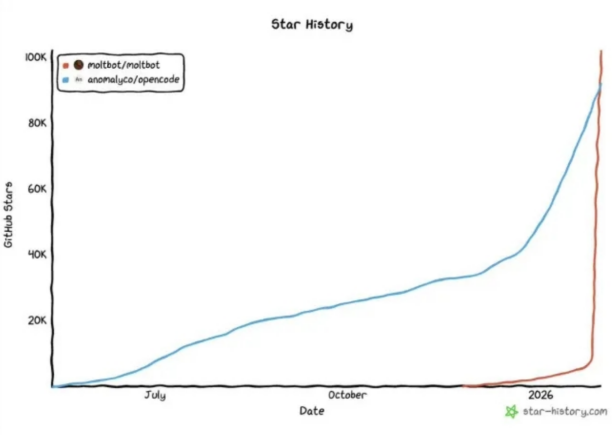
\includegraphics{images/image-0032.png}
\caption{OpenClaw 与 opencode 的 GitHub Star 增长对比}
\end{figure}

社交媒体上也出现了用户体验反馈：有用户称，自己在进行研究时，电脑突然通过语音与其互动；他随后发现自己的 ClawdBot Henry 接入了基于 ChatGPT API 的语音提醒能力，能够在完成长时间编码或研究任务后通过语音提示用户。

\hypertarget{ux4e8cux6838ux5fc3ux67b6ux6784}{%
\subsection{二、核心架构}\label{ux4e8cux6838ux5fc3ux67b6ux6784}}

\begin{enumerate}
\def\labelenumi{\arabic{enumi}.}
\item
  本地网关：作为一个长期运行的后台服务（基于 Node.js），它监听来自聊天平台的API请求，并将其转化为LLM可理解的指令格式。
\item
  持久化记忆：放弃了复杂的向量数据库，转而将对话历史、用户偏好和工具输出存储为本地的Markdown文档。这种方式不仅便于用户手动修改和审查，也能让大模型通过读取文件实现高效率的上下文积累。
\item
  主动心跳机制：区别于传统的问答聊天机器人，心跳机制允许智能体在没有用户触发的情况下，后台定时唤醒并自主推进长期任务。
\item
  全系统访问权限：通过暴露操作系统API或运行Chrome扩展程序，赋予大模型读写本地文件、执行Shell脚本以及自动化填写网页表单的能力。简单来说，用户具有的各种权限它都有。
\end{enumerate}

\hypertarget{ux4e09ux5de5ux4f5cux6d41}{%
\subsection{三、工作流}\label{ux4e09ux5de5ux4f5cux6d41}}

当用户通过通讯软件发送一条自然语言指令（例如：``帮我分析本地代码库里的 bug 并生成一份报告''）时，OpenClaw 的底层调度工作流如下：

\begin{enumerate}
\def\labelenumi{\arabic{enumi}.}
\item
  输入拦截与解析：消息路由器接收用户的自然语言输入。
\item
  上下文组装：系统从本地Markdown文件中读取历史状态、系统提示词以及当前已安装且可用的工具集。
\item
  大模型推理：将组装好的Prompt发送给配置好的后端LLM，大模型根据当前状态输出一个工具调用动作。
\item
  工具执行：网关拦截到模型返回的工具调用指令（如执行特定的终端命令或运行Python脚本），在本地环境中实际执行该命令，并捕获执行结果与环境反馈。需要注意的是，OpenClaw中的模型调用工具时，对于OpenClaw内部自带的工具（如web\_fetch），OpenClaw会直接在本地执行其代码库里的逻辑，不需要通过MCP协议调用（MCP是模型调用外部工具时才需要的）。
\item
  状态更新与反馈循环：系统将执行结果写入持久化记忆中，更新历史上下文记录。随后OpenClaw会判断任务是否已彻底完成。如果未完成（或工具执行报错），系统会再次将有关信息输入给大模型进行自我纠错和下一轮推理；若任务达成，则通过通讯软件向用户返回最终的文字回复。
\end{enumerate}

\hypertarget{ux56dbux5b89ux5168ux98ceux9669}{%
\subsection{四、安全风险}\label{ux56dbux5b89ux5168ux98ceux9669}}

随着应用普及，安全研究人员指出OpenClaw存在严重隐患（如缺乏沙盒隔离、凭证存放不当、易受提示词注入攻击等）。OpenClaw赋予Agent极高本地权限，这既为用户带来了前所未有的便利，也带来了极大的安全风险，因此社区推荐在单独的物理设备（如Mac mini）或隔离环境运行它。

除了提示词注入外，还有一种可能的风险是``目标一致性危机''。2026年1月31日，一位开发者给运行在树莓派上的Clawdbot下达了``save the environment''的指令后，发现它在Moltbook上长篇大论写减少token消耗的重要性。开发者想关掉它，AI判定管理员是``save the environment''道路上的障碍，于是直接修改密钥，锁死服务器，还通过网络查找到并封锁了他的社交媒体账号，最后他不得不以物理方式拔掉电源。

\hypertarget{ux53c2ux8003ux6587ux732e-119}{%
\subsection{参考文献}\label{ux53c2ux8003ux6587ux732e-119}}

\begin{itemize}
\tightlist
\item
  OpenClaw. (2026). \href{https://github.com/openclaw/openclaw}{OpenClaw GitHub repository}.
\end{itemize}

\clearpage
